\documentclass[oneside, doctor]{BIThesis}

\begin{document}

%%%%%%%%%%%%%%%%%%%%%%%%% 填写以下信息 %%%%%%%%%%%%%%%%%%%%%%%%%
\CLC{TQ028.1} % 中图分类号
\UDC{540} % UDC 分类号

\title{中国科研人员对开放获取期刊的认知、态度及行为研究} % 论文题目
\author{张三丰} % 作者姓名
\institute{材料学院} % 学院名称
\mentor{张亮教授} % 指导教师
\chairman{刘小明教授} % 答辩委员会主席
\degree{工学博士} % 申请学位
\major{材料科学与工程} % 学科专业
\school{北京理工大学} % 学位授予单位
\date{2009年6月} % 论文答辩日期

\englishtitle{Synthesis and Application on textile of the Shape Memory Polyurethane} % 论文题目(英)
\englishauthor{Ling Gao} % 作者姓名(英)
\englishinstitute{Material Science and Engineering} % 学院名称(英)
\englishmentor{Prof. Liang Zhang} % 指导教师(英)
\englishchairman{Prof. Xiaoming Liu} % 答辩委员会主席(英)
\englishdegree{Doctor of Philosophy} % 申请学位(英)
\englishmajor{Material Science and Engineering} % 学科专业(英)
\englishschool{Beijing Institute of Technology} % 学位授予单位(英)
\englishdate{June, 2009} % 论文答辩日期(英)
%%%%%%%%%%%%%%%%%%%%%%%%% 填写以上信息 %%%%%%%%%%%%%%%%%%%%%%%%%

\makecoverpage % 封面
\maketitlepage % 中文题名页
\makeenglishtitlepage % 英文题名页
\makeverticaltitlepage % 竖排题名页
\makedeclarationpage % 声明和授权页

\frontmatter

\begin{abstract}

本文……。({\color{blue}{摘要是一篇具有独立性和完整性的短文,应概括而扼要地反映出本论文的主要内容。
包括研究目的、研究方法、研究结果和结论等,特别要突出研究结果和结论。
中文摘要力求语言精炼准确,硕士学位论文摘要建议500$\sim$800字,博士学位论文建议1000$\sim$1200字。
摘要中不可出现参考文献、图、表、化学结构式、非公知公用的符号和术语。英文摘要与中文摘要的内容应一致,
在语法、用词上应准确无误,语言简练通顺。留学生的英文版博士学位论文中应有不少于3000字的“详细中文摘要”。}})

\keywords{形状记忆;聚氨酯;织物;合成;应用 ({\color{blue}{一般选3~6个单词或专业术语,
按词条的外延层次从大到小排列,之间用分号隔开,且中英文关键词必须对应。})}}

\end{abstract}

%%%%%%%%%%%%%%%%%%%%%%%%%%%%%%%%%%%%%%%%%%%%%%%%%%%%%%%%%%%%%%%%%%%%%%%%%%%%%%%%%%%%%%%%%%%%%%%%%%%%

\begin{englishabstract}

In order to exploit …….

\englishkeywords{shape memory properties; polyurethane; textile; synthesis; application}

\end{englishabstract}
 % 中英文摘要

\tableofcontents % 目录

\let\origaddvspace\addvspace
\renewcommand{\addvspace}[1]{}
\cleardoublepage
\pdfbookmark[0]{插图}{listoffigures}
\listoffigures % 插图
\cleardoublepage
\pdfbookmark[0]{附表}{listoftables}
\listoftables % 附表
\renewcommand{\addvspace}[1]{\origaddvspace{#1}}

\begin{denotation}

    \item[BIT] 北京理工大学的英文缩写
    \item[\LaTeX] 一个很棒的排版系统
    \item[\LaTeXe] 一个很棒的排版系统的最新稳定版
    \item[\XeTeX] \LaTeX{}的好兄弟,事实上他有很多个兄弟,但是这个兄弟对各种语言的支持能力都很强
    \item[ctex] 成套的中文\LaTeX{}解决方案,由一帮天才们开发
    \item[\ce{H2SO4}] 硫酸
    \item[$ e^{\pi{}i}+1=0$] 一个集自然界五大常数一体的炫酷方程
    \item[\ce{2H2 + O2 -> 2H2O}] 一个昂贵的生成生命之源的方程式

\end{denotation}
     % 注释表

\mainmatter

\chapter{绪论}
\label{chap:intro}
\section{本论文研究的目的和意义}

近年来,随着人们生活水平的不断提高,人们越来越注重周围环境对身体健康的影响。作为服装是人们时时刻刻最贴近的环境,尤其是内衣,对人体健康有很大的影响。由于合时刻刻最贴近的环境,尤其是内衣,对人体健康有很大的影响。由于合成纤维的衣着舒适性、手感性,天然纤维的发展又成为人们关注的一大热点。

……\upcite{Takahashi1996Structure, Xia2002Analysis, Jiang1989, Mao2000Motion, Feng1998}

\section{国内外研究现状及发展趋势}
%\label{sec:***} 可标注label

\subsection{形状记忆聚氨酯的形状记忆机理}
%\label{sec:features}

形状记忆聚合物(SMP)是继形状记忆合金后在80年代发展起来的一种新型形状记忆材料\upcite{Jiang1989}。形状记忆高分子材料在常温范围内具有塑料的性质,即刚性、形状稳定恢复性;同时在一定温度下(所谓记忆温度下)具有橡胶的特性,主要表现为材料的可变形性和形变恢复性。即“记忆初始态-固定变形-恢复起始态”的循环。

固定相只有物理交联结构的聚氨酯称为热塑性SMPU,而有化学交联结构称为热固性SMPU。热塑性和热固性形状记忆聚氨酯的形状记忆原理示意图如图\ref{fig:diagram}所示

\begin{figure}
    \centering
    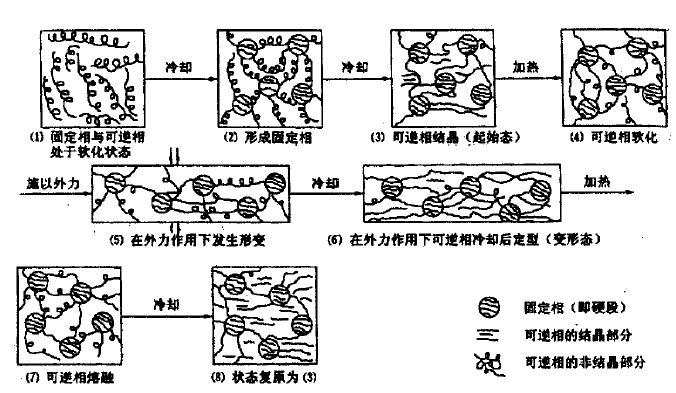
\includegraphics[width=0.75\textwidth]{figure/fig1}
    \caption{热塑性形状记忆聚氨酯的形状记忆机理示意图}\label{fig:diagram}
\end{figure}


\subsection{形状记忆聚氨酯的研究进展}
%\label{sec:requirements}
首例SMPU是日本Mitsubishi公司开发成功的……。

\subsection{水系聚氨酯及聚氨酯整理剂}

水系聚氨酯的形态对其流动性,成膜性及加工织物的性能有重要影响,一般分为三种类型\cite{Jiang2005Size} ,如表 \ref{tab:category}所示。

\begin{table}
    \centering
    \caption{水系聚氨酯分类} \label{tab:category}
    \begin{tabular*}{0.9\textwidth}{@{\extracolsep{\fill}}cccc}
        \toprule
        类别			&水溶型		&胶体分散型		&乳液型 \\
        \midrule
        状态			&溶解$\sim$胶束	&分散		&白浊 \\
        外观			&水溶型		&胶体分散型		&乳液型 \\
        粒径$/\mu m$	&$<0.001$		&$0.001-0.1$		&$>0.1$ \\
        重均分子量	&$1000\sim 10000$	&数千$\sim 20$万 &$>5000$ \\
        \bottomrule
    \end{tabular*}
\end{table}

由于它们对纤维织物的浸透性和亲和性不同,因此在纺织品染整加工中的用途也有差别,其中以水溶型和乳液型产品较为常用。另外,水系聚氨酯又有反应性和非反应性之分。虽然它们的共同特点是分子结构中不含异氰酸酯基,但前者是用封闭剂将异氰酸酯基暂时封闭,在纺织品整理时复出。相互交联反应形成三维网状结构而固着在织物表面。
…… % 第一章
\input{main/03_chapter2} % 第二章
\input{main/04_chapter3} % 第三章
\input{main/05_chapter4} % 第四章
\input{main/06_chapter5} % 第五章
\begin{conclusion}

本文采用……。{\color{blue}(结论作为学位论文正文的最后部分单独排写,但不加章号。结论是对整个论文主要结果的总结。
在结论中应明确指出本研究的创新点,对其应用前景和社会、经济价值等加以预测和评价,并指出今后进一步在本研究方向进行研究工作的展望与设想。
结论部分的撰写应简明扼要,突出创新性。)}

\end{conclusion} % 结论
\bibliography{reference/ref} % 参考文献

\appendix
\renewcommand{\theequation}{\Alph{chapter}--\arabic{equation}}
\renewcommand{\thefigure}{\Alph{chapter}--\arabic{figure}}
\renewcommand{\thetable}{\Alph{chapter}--\arabic{table}}

\chapter{***}

附录相关内容…
 % 附录一
\chapter{Maxwell Equations}

因为在柱坐标系下,$\overline{\overline\mu}$是对角的,所以Maxwell方程组中电场$\bf
    E$的旋度

所以$\bf H$的各个分量可以写为:
\begin{subequations}
    \begin{eqnarray}
        H_r=\frac{1}{\mathbf{i}\omega\mu_r}\frac{1}{r}\frac{\partial
            E_z}{\partial\theta } \\
        H_\theta=-\frac{1}{\mathbf{i}\omega\mu_\theta}\frac{\partial E_z}{\partial r}
    \end{eqnarray}
\end{subequations}
同样地,在柱坐标系下,$\overline{\overline\epsilon}$是对角的,所以Maxwell方程组中磁场$\bf
    H$的旋度
\begin{subequations}
    \begin{eqnarray}
        &&\nabla\times{\bf H}=-\mathbf{i}\omega{\bf D}\\
        &&\left[\frac{1}{r}\frac{\partial}{\partial
                r}(rH_\theta)-\frac{1}{r}\frac{\partial
                H_r}{\partial\theta}\right]{\hat{\bf
                z}}=-\mathbf{i}\omega{\overline{\overline\epsilon}}{\bf
            E}=-\mathbf{i}\omega\epsilon_zE_z{\hat{\bf z}} \\
        &&\frac{1}{r}\frac{\partial}{\partial
            r}(rH_\theta)-\frac{1}{r}\frac{\partial
            H_r}{\partial\theta}=-\mathbf{i}\omega\epsilon_zE_z
    \end{eqnarray}
\end{subequations}
由此我们可以得到关于$E_z$的波函数方程:
\begin{eqnarray}
    \frac{1}{\mu_\theta\epsilon_z}\frac{1}{r}\frac{\partial}{\partial r}
    \left(r\frac{\partial E_z}{\partial r}\right)+
    \frac{1}{\mu_r\epsilon_z}\frac{1}{r^2}\frac{\partial^2E_z}{\partial\theta^2}
    +\omega^2 E_z=0
\end{eqnarray}
 % 附录二

\backmatter

\begin{publications}{99}

    \item{高凌}. {交联型与线形水性聚氨酯的形状记忆性能比较}[J].
    化工进展, 2006, 532-535.(核心期刊)

\end{publications}
 % 论文和研究成果清单
\begin{acknowledgment}

    本论文的工作是在导师……。

\end{acknowledgment} % 致谢
\begin{resume}

    本人…。

\end{resume} % 作者简介

\end{document}
